% !TEX program = pdflatex
\documentclass[a4paper,12pt]{article}
\usepackage[utf8]{inputenc}
\usepackage[T1]{fontenc}
\usepackage[margin=2.2cm]{geometry}
\usepackage{amsmath,hyperref,xcolor,tikz,listings,tcolorbox,fontawesome5}
\usepackage{fancyhdr,tocloft,enumitem,tabularx,booktabs}
\usetikzlibrary{shapes.geometric,arrows.meta,positioning,calc,fit,backgrounds,shadows,decorations.pathreplacing}
\tcbuselibrary{skins,breakable}

\definecolor{bg}{HTML}{0a0e17}\definecolor{fg}{HTML}{c0c0c0}\definecolor{accent}{HTML}{00ffaa}
\definecolor{pink}{HTML}{ff66cc}\definecolor{red}{HTML}{e94560}\definecolor{orange}{HTML}{ffaa00}
\definecolor{darkbg}{HTML}{1a1a2e}\definecolor{mediumbg}{HTML}{161b22}\definecolor{border}{HTML}{2a2a3c}

\lstdefinestyle{bash}{basicstyle=\ttfamily\footnotesize\color{accent},backgroundcolor=\color{darkbg},frame=single,framerule=0.5pt,rulecolor=\color{red},breaklines=true}
\lstdefinestyle{json}{basicstyle=\ttfamily\footnotesize\color{fg},stringstyle=\color{accent},backgroundcolor=\color{darkbg},frame=single,framerule=0.5pt,rulecolor=\color{red},breaklines=true}
\lstdefinestyle{python}{basicstyle=\ttfamily\footnotesize\color{fg},keywordstyle=\color{pink},stringstyle=\color{accent},backgroundcolor=\color{darkbg},frame=single,framerule=0.5pt,rulecolor=\color{red},breaklines=true}

\newtcolorbox{infobox}[1][]{colback=darkbg,colframe=red,coltitle=fg,fonttitle=\bfseries,title=#1,arc=4pt,boxrule=1pt}

\pagestyle{fancy}\fancyhf{}\fancyhead[L]{\textcolor{accent}{\textbf{MagistralaCAN4 — REST API}}}
\fancyhead[R]{\textcolor{pink}{Dokumentacja}}\fancyfoot[C]{\textcolor{fg!50}{\thepage}}
\renewcommand{\headrulewidth}{1pt}\renewcommand{\headrule}{\hbox to\headwidth{\color{red}\leaders\hrule height \headrulewidth\hfill}}
\setlength{\headheight}{15pt}

\hypersetup{colorlinks=true,linkcolor=accent,urlcolor=pink}

\title{\vspace{-2cm}{\Huge\color{accent}\textbf{REST API}}\\[6pt]{\Large\color{pink}MagistralaCAN4}\\[4pt]{\normalsize\color{fg}Zdalne sterowanie i monitoring przez HTTP}\\[10pt]{\small\color{orange}Port 8080 \,|\, JSON \,|\, QTcpServer}}
\author{\color{fg}CustomLabs}
\date{\color{fg}\today}

\begin{document}
\maketitle\thispagestyle{empty}

\begin{tikzpicture}[overlay,remember picture]
\draw[red,line width=1.5pt]([shift={(-1cm,0.5cm)}]current page.south west)--([shift={(1cm,0.5cm)}]current page.south east);
\draw[accent,line width=0.5pt]([shift={(-1cm,0.2cm)}]current page.south west)--([shift={(1cm,0.2cm)}]current page.south east);
\end{tikzpicture}

\vfill\begin{center}\color{fg!70}\footnotesize\faServer\ HTTP \,|\, \faCode\ JSON \,|\, \faPlug\ Integracja\end{center}
\newpage
\tableofcontents
\newpage

% ═══════════════════════════════════════════════ 
\section{Co to jest REST API?}
% ═══════════════════════════════════════════════

REST (Representational State Transfer) API to interfejs komunikacyjny oparty na protokole \textbf{HTTP}. Działa na zasadzie żądań i odpowiedzi — klient wysyła zapytanie (GET, POST), serwer zwraca dane w formacie \textbf{JSON}.

W MagistralaCAN4 REST API nasłuchuje na porcie \textbf{8080} i udostępnia cztery endpointy:

\begin{center}
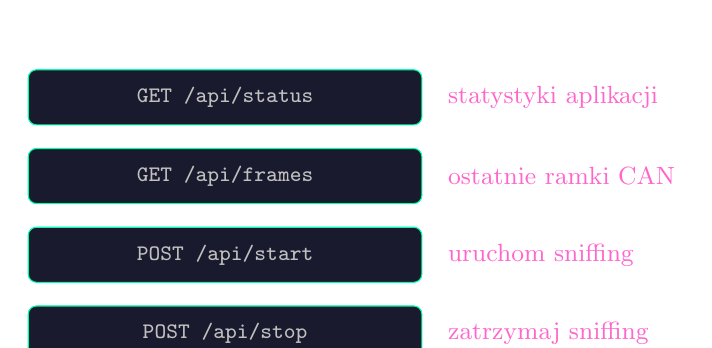
\begin{tikzpicture}[
    ep/.style={rectangle,draw=accent,fill=darkbg,text=fg,rounded corners=3pt,minimum width=5cm,minimum height=0.7cm,align=center,font=\footnotesize\ttfamily},
    arrow/.style={->,>=Stealth,line width=0.8pt,color=red}]
\node[ep] (s) at(0,0) {GET /api/status};
\node[ep] (f) at(0,-1){GET /api/frames};
\node[ep] (a) at(0,-2){POST /api/start};
\node[ep] (o) at(0,-3){POST /api/stop};
\node[font=\small\color{pink},right=0.2cm of s]{statystyki aplikacji};
\node[font=\small\color{pink},right=0.2cm of f]{ostatnie ramki CAN};
\node[font=\small\color{pink},right=0.2cm of a]{uruchom sniffing};
\node[font=\small\color{pink},right=0.2cm of o]{zatrzymaj sniffing};
\end{tikzpicture}
\end{center}

% ═══════════════════════════════════════════════ 
\section{Dlaczego REST API jest ważne?}
% ═══════════════════════════════════════════════

\subsection{Zdalne sterowanie}

\begin{lstlisting}[style=bash,caption={Zdalne uruchomienie sniffingu przez curl}]
curl -X POST http://192.168.1.10:8080/api/start
curl http://192.168.1.10:8080/api/status
\end{lstlisting}

\subsection{Integracja z zewnętrznymi systemami}

\begin{center}
\begin{tikzpicture}[
    sys/.style={rectangle,draw=pink,fill=darkbg,text=fg,rounded corners=3pt,minimum width=3cm,minimum height=0.8cm,align=center,font=\footnotesize},
    arrow/.style={<->,>=Stealth,line width=0.8pt,color=orange}]
\node[sys] (api) at(0,0) {REST API\\MagistralaCAN4};
\node[sys] (db) at(-4,2) {Dashboard\\Grafana/HTML};
\node[sys] (py) at(0,2.5) {Python\\skrypty};
\node[sys] (mon) at(4,2) {Monitoring\\Prometheus};
\node[sys] (mob) at(-4,-1.5) {Telefon\\przeglądarka};
\draw[arrow](api)--(db);\draw[arrow](api)--(py);\draw[arrow](api)--(mon);\draw[arrow](api)--(mob);
\end{tikzpicture}
\end{center}

\subsection{Lekkość i prostota}

REST API w MagistralaCAN4 to tylko $\sim$100 linii kodu (\texttt{HttpRestServer}), żadnych zewnętrznych zależności.

\subsection{Uzupełnienie WebSocket}

\begin{center}
\begin{tabularx}{0.9\textwidth}{@{}>{\color{accent}\bfseries}lX@{}}
\toprule\rowcolor{darkbg} Cecha & Opis \\\midrule
WebSocket & Strumień ciągły, JSON dla każdej ramki, port 9000 (WSS) \\
REST API  & Żądanie→odpowiedź, JSON agregowany, port 8080 (HTTP) \\
\bottomrule
\end{tabularx}
\end{center}

% ═══════════════════════════════════════════════ 
\section{Dlaczego warto tego używać?}
% ═══════════════════════════════════════════════

\subsection{Scenariusz 1 — Warsztat}

\begin{center}
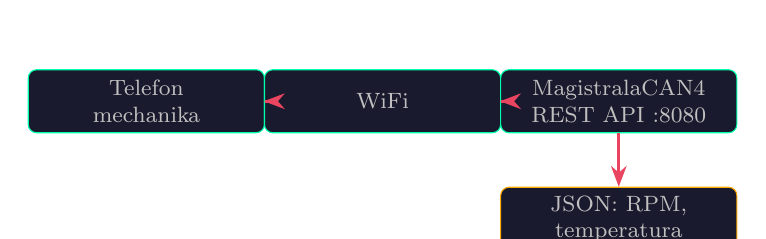
\begin{tikzpicture}[
    dev/.style={rectangle,draw=accent,fill=darkbg,text=fg,rounded corners=3pt,minimum width=3cm,minimum height=0.8cm,align=center,font=\footnotesize},
    arrow/.style={->,>=Stealth,line width=1pt,color=red}]
\node[dev](phone)at(-3,0) {Telefon\\mechanika};
\node[dev](wifi)at(0,0) {WiFi};
\node[dev](mag)at(3,0) {MagistralaCAN4\\REST API :8080};
\node[dev,draw=orange](data)at(3,-1.5) {JSON: RPM,\\temperatura};
\draw[arrow](phone)--(wifi);\draw[arrow](wifi)--(mag);\draw[arrow](mag)--(data);
\end{tikzpicture}
\end{center}

\subsection{Scenariusz 2 — Automatyzacja testów}

\begin{lstlisting}[style=python,caption={Automatyzacja testów w Pythonie}]
import requests, time
requests.post("http://localhost:8080/api/start")
time.sleep(10)
data = requests.get("http://localhost:8080/api/frames").json()
requests.post("http://localhost:8080/api/stop")
print(f"Zebrano {len(data)} ramek")
\end{lstlisting}

\subsection{Scenariusz 3 — Monitoring 24/7}

Co 30 sekund sprawdza \texttt{/api/status} i alarmuje gdy FPS spadnie poniżej progu.

% ═══════════════════════════════════════════════ 
\section{Jak używać — krok po kroku}
% ═══════════════════════════════════════════════

\subsection{Krok 1: Uruchom REST API}

W MagistralaCAN4 kliknij przycisk \texttt{[REST] REST API} w górnym toolbarze. Serwer nasłuchuje na porcie \textbf{8080}.

\subsection{Krok 2: Sprawdź status}

\begin{lstlisting}[style=bash,caption={curl /api/status}]
curl http://localhost:8080/api/status
\end{lstlisting}

\begin{lstlisting}[style=json,caption={Odpowiedź JSON}]
{
  "running": true,
  "frames": 1247,
  "fps": 82.0,
  "uniqueIds": 12
}
\end{lstlisting}

\begin{center}
\begin{tabularx}{0.8\textwidth}{@{}>{\color{accent}\ttfamily}lX@{}}
\toprule\rowcolor{darkbg} Pole & Znaczenie \\\midrule
running & Czy sniffing jest aktywny \\
frames & Liczba ramek w tabeli \\
fps & Ramki na sekundę (średnia z 500ms) \\
uniqueIds & Liczba unikalnych CAN ID \\
\bottomrule
\end{tabularx}
\end{center}

\subsection{Krok 3: Pobierz ramki}

\begin{lstlisting}[style=bash,caption={curl /api/frames}]
curl http://localhost:8080/api/frames
\end{lstlisting}

\subsection{Krok 4: Steruj sniffingiem}

\begin{lstlisting}[style=bash,caption={Start / Stop}]
curl -X POST http://localhost:8080/api/start
curl -X POST http://localhost:8080/api/stop
\end{lstlisting}

\subsection{Krok 5: Dashboard HTML}

\begin{lstlisting}[style=json,caption={Prosty dashboard w HTML/JS}]
<!DOCTYPE html><html><body>
<h1>MagistralaCAN4</h1><div id="status"></div>
<script>
setInterval(async () => {
  const r = await fetch('http://192.168.1.10:8080/api/status');
  const d = await r.json();
  document.getElementById('status').innerHTML =
    `Ramki: ${d.frames} | FPS: ${d.fps}`;
}, 1000);
</script></body></html>
\end{lstlisting}

% ═══════════════════════════════════════════════ 
\section{Architektura techniczna}
% ═══════════════════════════════════════════════

\begin{figure}[h!]
\centering
\begin{tikzpicture}[
    box/.style={rectangle,draw=accent,fill=darkbg,text=fg,rounded corners=4pt,minimum width=4cm,minimum height=1cm,align=center,font=\footnotesize,line width=1pt},
    arrow/.style={->,>=Stealth,line width=1pt,color=red}]
\node[box,draw=orange](client)at(-5,0){Klient\\curl / przeglądarka / Python};
\node[box,draw=pink](http)at(0,0){HTTP GET/POST\\JSON response};
\node[box,draw=accent](server)at(5,0){HttpRestServer\\(QTcpServer, port 8080)};
\node[box,draw=accent](model)at(5,-2){CanFrameModel\\(dane ramek CAN)};
\node[box,draw=pink](start)at(2.5,-2){toggleSniffing()\\(sterowanie)};
\draw[arrow](client)--(http);\draw[arrow](http)--(server);
\draw[arrow](server)--(model);\draw[arrow,dashed,color=orange](server)--(start);
\node[font=\footnotesize\color{fg!60},below=0.2cm of model]{dostarcza ramki i statystyki};
\node[font=\footnotesize\color{fg!60},below=0.2cm of start]{emituje sygnał start/stop};
\end{tikzpicture}
\caption{Architektura REST API — przepływ żądania}
\end{figure}

\begin{center}
\begin{tikzpicture}[
    layer/.style={rectangle,draw=border,fill=darkbg,text=fg,rounded corners=3pt,minimum width=5.5cm,minimum height=0.7cm,align=center,font=\footnotesize},
    arrow/.style={->,>=Stealth,line width=0.8pt,color=accent}]
\node[layer,draw=red](tcp)at(0,2){QTcpServer — nasłuchuje na 0.0.0.0:8080};
\node[layer,draw=orange](parse)at(0,1){Parser HTTP — metoda + ścieżka};
\node[layer,draw=accent](route)at(0,0){Routing — /api/status, /api/frames, ...};
\node[layer,draw=pink](handler)at(0,-1){Handler — CanFrameModel, sygnały start/stop};
\node[layer,draw=accent](json)at(0,-2){JSON response — HTTP 200};
\draw[arrow](tcp)--(parse);\draw[arrow](parse)--(route);
\draw[arrow](route)--(handler);\draw[arrow](handler)--(json);
\node[font=\footnotesize\color{fg!60},right=0.3cm of tcp]{akceptuje połączenia TCP};
\node[font=\footnotesize\color{fg!60},right=0.3cm of parse]{GET /api/status HTTP/1.1};
\node[font=\footnotesize\color{fg!60},right=0.3cm of route]{dopasowuje ścieżkę};
\node[font=\footnotesize\color{fg!60},right=0.3cm of handler]{zbiera dane};
\node[font=\footnotesize\color{fg!60},right=0.3cm of json]{Content-Type: application/json};
\end{tikzpicture}
\end{center}

% ═══════════════════════════════════════════════ 
\section{Endpointy — pełne zestawienie}
% ═══════════════════════════════════════════════

\begin{center}
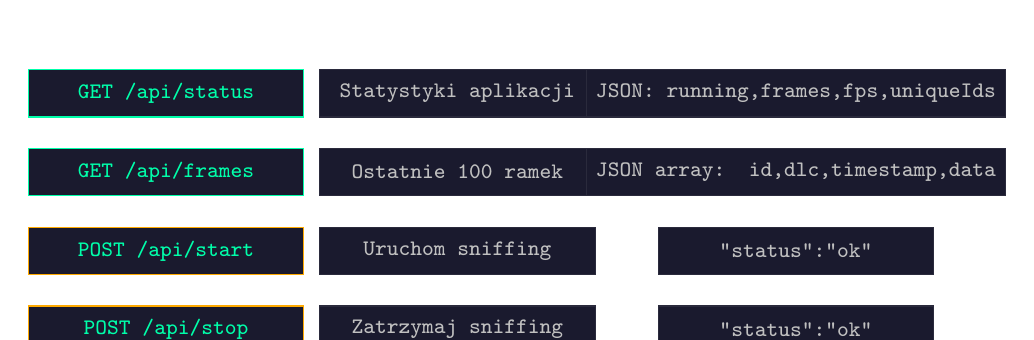
\begin{tikzpicture}[
    row/.style={rectangle,draw=border,fill=darkbg,text=fg,minimum width=3.5cm,minimum height=0.6cm,align=center,font=\footnotesize\ttfamily},
    highlight/.style={rectangle,draw=accent,fill=darkbg,text=accent,minimum width=3.5cm,minimum height=0.6cm,align=center,font=\footnotesize\ttfamily\bfseries}]
\node[highlight]at(-5.5,0){GET /api/status};
\node[row]at(-1.8,0){Statystyki aplikacji};
\node[row]at(2.5,0){JSON: running,frames,fps,uniqueIds};

\node[highlight]at(-5.5,-1){GET /api/frames};
\node[row]at(-1.8,-1){Ostatnie 100 ramek};
\node[row]at(2.5,-1){JSON array: id,dlc,timestamp,data};

\node[highlight,draw=orange]at(-5.5,-2){POST /api/start};
\node[row]at(-1.8,-2){Uruchom sniffing};
\node[row]at(2.5,-2){{"status":"ok"}};

\node[highlight,draw=orange]at(-5.5,-3){POST /api/stop};
\node[row]at(-1.8,-3){Zatrzymaj sniffing};
\node[row]at(2.5,-3){{"status":"ok"}};
\end{tikzpicture}
\end{center}

% ═══════════════════════════════════════════════ 
\section{Bezpieczeństwo}
% ═══════════════════════════════════════════════

\begin{itemize}[nosep]
\item REST API nasłuchuje na \texttt{0.0.0.0:8080} — dostępne z sieci
\item Brak wbudowanej autoryzacji (założenie: zaufana sieć LAN)
\item Ograniczenie przez firewall: \texttt{sudo ufw allow from 192.168.1.0/24 to any port 8080}
\item Przyszłościowo: token \texttt{Authorization: Bearer <token>}
\end{itemize}

\vfill
\begin{center}

\begin{tikzpicture}
\draw[red,line width=1.5pt](0,0)--(\textwidth-2cm,0);
\draw[accent,line width=0.5pt](0,-0.3)--(\textwidth-2cm,-0.3);
\node[font=\footnotesize\color{fg!60},above=0.4cm]at(\textwidth/2-1cm,0){© 2025--2026 CustomLabs \,|\, MagistralaCAN4 REST API};
\end{tikzpicture}
\end{center}
\end{document}
